% Projeto Integrador AOC 2026/02 --- artigo final (formato IEEE, em inglês)
% Compilar: latexmk -pdf artigo.tex     (ou, na raiz do repositório: make paper)
% As figuras de erro leem os dados de ../../results/, gerados por: make bench
\documentclass[conference]{IEEEtran}

\usepackage[T1]{fontenc}
\usepackage[utf8]{inputenc}
\usepackage{amsmath,amssymb}
\usepackage{booktabs}
\usepackage{cite}
\usepackage{xcolor}
\usepackage{tikz}
\usetikzlibrary{arrows.meta,positioning,calc}
\usepackage{pgfplots}
\usepgfplotslibrary{groupplots}
\pgfplotsset{compat=1.18}
\usepackage[hidelinks]{hyperref}

\newcommand{\code}[1]{\texttt{#1}}
\newcommand{\res}{../../results}
\newcommand{\cdf}[3][]{\addplot+[no markers, #1] table[x=err, y=frac] {\res/cdf_#2_#3.dat};}

% Gerado por: python3 -m sim.paper_numbers (não editar à mão)
\newcommand{\ERRTABLE}{T8 & \boldmath$1.6\times10^{0}$ & $6.8\times10^{-2}$ & \boldmath$2.1\times10^{-1}$ & $7.7\times10^{-2}$ & $1.1\times10^{-1}$ & $1.4\times10^{-1}$ & $5.7\times10^{-2}$ & \boldmath$5.4\times10^{-1}$ & $1.4\times10^{-1}$\\
FP8 & $1.6\times10^{0}$ & $7.7\times10^{-2}$ & $\infty$ & $9.0\times10^{-2}$ & $5.4\times10^{-2}$ & $6.4\times10^{-2}$ & $4.4\times10^{-2}$ & $\infty$ & $7.2\times10^{-2}$\\
FP8w & $1.7\times10^{0}$ & \boldmath$4.4\times10^{-2}$ & $\infty$ & \boldmath$4.1\times10^{-2}$ & \boldmath$3.8\times10^{-2}$ & \boldmath$5.1\times10^{-2}$ & \boldmath$3.6\times10^{-2}$ & $\infty$ & \boldmath$6.4\times10^{-2}$\\
\midrule
T16 & \boldmath$6.9\times10^{-3}$ & \boldmath$2.7\times10^{-4}$ & $8.4\times10^{-4}$ & \boldmath$2.5\times10^{-4}$ & \boldmath$2.6\times10^{-4}$ & $5.4\times10^{-4}$ & \boldmath$2.3\times10^{-4}$ & \boldmath$2.0\times10^{-3}$ & $5.8\times10^{-4}$\\
FP16 & $9.1\times10^{-3}$ & $4.7\times10^{-4}$ & $3.8\times10^{-4}$ & $6.7\times10^{-4}$ & $3.9\times10^{-4}$ & $3.5\times10^{-4}$ & $2.9\times10^{-4}$ & $\infty$ & $3.8\times10^{-4}$\\
FP16w & $9.0\times10^{-3}$ & $3.2\times10^{-4}$ & \boldmath$2.4\times10^{-4}$ & $3.2\times10^{-4}$ & $3.0\times10^{-4}$ & \boldmath$3.1\times10^{-4}$ & $2.4\times10^{-4}$ & $\infty$ & \boldmath$3.1\times10^{-4}$\\
\midrule
T32 & \boldmath$9.9\times10^{-8}$ & \boldmath$4.2\times10^{-9}$ & \boldmath$1.4\times10^{-8}$ & \boldmath$3.4\times10^{-9}$ & \boldmath$3.7\times10^{-9}$ & \boldmath$8.3\times10^{-9}$ & \boldmath$3.8\times10^{-9}$ & \boldmath$3.3\times10^{-8}$ & \boldmath$8.6\times10^{-9}$\\
FP32 & $1.2\times10^{-6}$ & $6.9\times10^{-8}$ & $5.2\times10^{-8}$ & $1.0\times10^{-7}$ & $4.6\times10^{-8}$ & $5.2\times10^{-8}$ & $3.7\times10^{-8}$ & $6.2\times10^{-8}$ & $4.8\times10^{-8}$\\
FP32w & $9.3\times10^{-7}$ & $4.3\times10^{-8}$ & $3.1\times10^{-8}$ & $3.8\times10^{-8}$ & $3.5\times10^{-8}$ & $3.8\times10^{-8}$ & $3.0\times10^{-8}$ & $4.0\times10^{-8}$ & $3.8\times10^{-8}$\\}
\newcommand{\ERRTABLESYN}{T8 & \boldmath$1.6\times10^{0}$ & $6.8\times10^{-2}$ & \boldmath$2.1\times10^{-1}$ & $7.7\times10^{-2}$\\
FP8 & $1.6\times10^{0}$ & $7.7\times10^{-2}$ & $\infty$ & $9.0\times10^{-2}$\\
FP8w & $1.7\times10^{0}$ & \boldmath$4.4\times10^{-2}$ & $\infty$ & \boldmath$4.1\times10^{-2}$\\
\midrule
T16 & \boldmath$6.9\times10^{-3}$ & \boldmath$2.7\times10^{-4}$ & $8.4\times10^{-4}$ & \boldmath$2.5\times10^{-4}$\\
FP16 & $9.1\times10^{-3}$ & $4.7\times10^{-4}$ & $3.8\times10^{-4}$ & $6.7\times10^{-4}$\\
FP16w & $9.0\times10^{-3}$ & $3.2\times10^{-4}$ & \boldmath$2.4\times10^{-4}$ & $3.2\times10^{-4}$\\
\midrule
T32 & \boldmath$9.9\times10^{-8}$ & \boldmath$4.2\times10^{-9}$ & \boldmath$1.4\times10^{-8}$ & \boldmath$3.4\times10^{-9}$\\
FP32 & $1.2\times10^{-6}$ & $6.9\times10^{-8}$ & $5.2\times10^{-8}$ & $1.0\times10^{-7}$\\
FP32w & $9.3\times10^{-7}$ & $4.3\times10^{-8}$ & $3.1\times10^{-8}$ & $3.8\times10^{-8}$\\}
\newcommand{\ERRTABLEREAL}{T8 & $1.1\times10^{-1}$ & $1.4\times10^{-1}$ & $5.7\times10^{-2}$ & \boldmath$5.4\times10^{-1}$ & $1.4\times10^{-1}$\\
FP8 & $5.4\times10^{-2}$ & $6.4\times10^{-2}$ & $4.4\times10^{-2}$ & $\infty$ & $7.2\times10^{-2}$\\
FP8w & \boldmath$3.8\times10^{-2}$ & \boldmath$5.1\times10^{-2}$ & \boldmath$3.6\times10^{-2}$ & $\infty$ & \boldmath$6.4\times10^{-2}$\\
\midrule
T16 & \boldmath$2.6\times10^{-4}$ & $5.4\times10^{-4}$ & \boldmath$2.3\times10^{-4}$ & \boldmath$2.0\times10^{-3}$ & $5.8\times10^{-4}$\\
FP16 & $3.9\times10^{-4}$ & $3.5\times10^{-4}$ & $2.9\times10^{-4}$ & $\infty$ & $3.8\times10^{-4}$\\
FP16w & $3.0\times10^{-4}$ & \boldmath$3.1\times10^{-4}$ & $2.4\times10^{-4}$ & $\infty$ & \boldmath$3.1\times10^{-4}$\\
\midrule
T32 & \boldmath$3.7\times10^{-9}$ & \boldmath$8.3\times10^{-9}$ & \boldmath$3.8\times10^{-9}$ & \boldmath$3.3\times10^{-8}$ & \boldmath$8.6\times10^{-9}$\\
FP32 & $4.6\times10^{-8}$ & $5.2\times10^{-8}$ & $3.7\times10^{-8}$ & $6.2\times10^{-8}$ & $4.8\times10^{-8}$\\
FP32w & $3.5\times10^{-8}$ & $3.8\times10^{-8}$ & $3.0\times10^{-8}$ & $4.0\times10^{-8}$ & $3.8\times10^{-8}$\\}
\newcommand{\RATA}{1.2}
\newcommand{\RATB}{11}
\newcommand{\WIDET}{$8.4\times10^{-4}$}
\newcommand{\WIDEF}{$2.4\times10^{-4}$}
\newcommand{\BUST}{$5.4\times10^{-4}$}
\newcommand{\BUSF}{$3.1\times10^{-4}$}
\newcommand{\WIDETEIGHT}{$2.1\times10^{-1}$}
\newcommand{\BCSTEIGHT}{$5.4\times10^{-1}$}
\newcommand{\BCSTSIXTEEN}{$2.0\times10^{-3}$}
\newcommand{\FPEIGHTBAD}{217}
\newcommand{\NFBUS}{94}
\newcommand{\NFWEST}{51}
\newcommand{\NFBCS}{153}
\newcommand{\NFWESTH}{5}
\newcommand{\NFBCSH}{149}
\newcommand{\MEMTE}{$1.4\times10^{-1}$}
\newcommand{\MEMTEBAD}{267}
\newcommand{\MEMFE}{$6.4\times10^{-2}$}
\newcommand{\MEMFEBAD}{1\,054}
\newcommand{\MEMTS}{$5.8\times10^{-4}$}
\newcommand{\MEMTSBAD}{3}
\newcommand{\MEMFS}{$3.1\times10^{-4}$}
\newcommand{\MEMFSBAD}{2}
\newcommand{\MEMTT}{$8.6\times10^{-9}$}
\newcommand{\MEMTTBAD}{0}
\newcommand{\MEMFT}{$3.8\times10^{-8}$}
\newcommand{\MEMFTBAD}{0}
\newcommand{\MEMROWS}{17\,758}
\newcommand{\MATTABLE}{poisson & 256$\times$256 & 1\,216 & 4.8 & $2^{0}$ -- $2^{2}$\\
gauss & 256$\times$256 & 2\,560 & 10.0 & $2^{-13}$ -- $2^{2}$\\
wide & 256$\times$256 & 2\,560 & 10.0 & $2^{-10}$ -- $2^{10}$\\
mlp & 256$\times$512 & 13\,056 & 51.0 & $2^{-15}$ -- $2^{0}$\\
\midrule
nos4 & 100$\times$100 & 594 & 5.9 & $2^{-6}$ -- $2^{-1}$\\
bus494 & 494$\times$494 & 1\,666 & 3.4 & $2^{-3}$ -- $2^{14}$\\
west0479 & 479$\times$479 & 1\,910 & 4.0 & $2^{-21}$ -- $2^{18}$\\
bcsstk05 & 153$\times$153 & 2\,423 & 15.8 & $2^{-31}$ -- $2^{22}$\\
memplus & 17758$\times$17758 & 126\,150 & 7.1 & $2^{-86}$ -- $2^{0}$\\}
\newcommand{\INSTRTABLE}{poisson & 4.8 & 6\,146 & 6\,146 & 6\,658 & 0.0\% & 7.7\%\\
gauss & 10.0 & 8\,962 & 9\,218 & 9\,986 & 2.8\% & 10.3\%\\
mlp & 51.0 & 23\,042 & 24\,578 & 26\,626 & 6.2\% & 13.5\%\\
\midrule
nos4 & 5.9 & 2\,402 & 2\,402 & 2\,602 & 0.0\% & 7.7\%\\
bus494 & 3.4 & 11\,902 & 11\,906 & 12\,898 & 0.0\% & 7.7\%\\
west0479 & 4.0 & 11\,949 & 11\,990 & 12\,989 & 0.3\% & 8.0\%\\
bcsstk05 & 15.8 & 6\,061 & 6\,278 & 6\,801 & 3.5\% & 10.9\%\\
memplus & 7.1 & 503\,161 & 510\,158 & 552\,671 & 1.4\% & 9.0\%\\}
\newcommand{\SAVEWLO}{7.7}
\newcommand{\SAVEWHI}{14.3}
\newcommand{\SAVEPHI}{7.1}
\newcommand{\FLAGPCT}{90}
\newcommand{\FLAGWHERE}{\emph{wide}, FP32}
\newcommand{\HWDECA}{46}
\newcommand{\HWDECB}{89}
\newcommand{\HWDECC}{164}
\newcommand{\HWENCA}{70}
\newcommand{\HWENCB}{118}
\newcommand{\HWENCC}{216}
\newcommand{\HWALUA}{327}
\newcommand{\HWALUB}{912}
\newcommand{\HWALUC}{2\,838}
\newcommand{\HWNCA}{32}
\newcommand{\HWNCB}{67}
\newcommand{\HWNCC}{155}
\newcommand{\HWWMA}{220}
\newcommand{\HWWMB}{686}
\newcommand{\HWWMC}{2\,384}
\newcommand{\HWDOTA}{6\,740}
\newcommand{\HWDOTB}{7\,525}
\newcommand{\HWDOTC}{9\,451}
\newcommand{\HWHDR}{41}

\newcommand{\matplot}[2][]{%
  \nextgroupplot[title={#2}, #1]
  \cdf[blue!75!black]{#2}{T8}    \cdf[blue!75!black, dashed]{#2}{FP8w}
  \cdf[red!75!black]{#2}{T16}    \cdf[red!75!black, dashed]{#2}{FP16w}
  \cdf[green!45!black]{#2}{T32}  \cdf[green!45!black, dashed]{#2}{FP32w}}

\begin{document}

\title{Zvtakum: Takum Arithmetic in the RISC-V Vector Extension\\
{\large RTL Datapath, Instruction-Level Simulation and Sparse Linear Algebra Evaluation}}

\author{\IEEEauthorblockN{Heloisa Silva Rosa, Samantha Kelly de Souza Sena and Vitor Hugo Lacerda Lana}
\IEEEauthorblockA{Departamento de Engenharia Eletr\^onica (DELT), Universidade Federal de Minas Gerais\\
Belo Horizonte, MG, Brazil}}

\maketitle

\begin{abstract}
Vector instruction sets keep adding low-precision IEEE~754-style formats, each with its own decoding
logic, exception cases and control state. Takum arithmetic is a tapered-precision alternative whose
header is decoded from at most 12 bits at any width. We present Zvtakum, a simplified takum extension
for the RISC-V vector extension with five instructions (\code{vtadd.vv}, \code{vtsub.vv},
\code{vtmul.vv}, \code{vtdot.vv}, \code{vncvt.t.t}) for 8-, 16- and 32-bit elements. We describe a
Verilog datapath, verified against an exact rational oracle (exhaustively at 8 bits), and an
instruction-level simulator that executes the encoded instructions together with a subset of RVV.
On sparse matrix--vector products with nine matrices, five of them from the public Matrix Market
repository and one with 17\,758 rows,
compared with a binary128 reference, 32-bit takums have the lowest median relative error in every case,
up to 11 times lower than binary32 with the same accumulation precision; 16-bit takums win on data near
unit scale, lose on moderately wide ranges and stay finite where binary16 overflows; and 8-bit takums are
less precise than an 8-bit float on in-range data but never overflow, whereas the float returns
infinities or NaN for 11\% to 100\% of the rows of four matrices. The fused dot-product instruction removes 8--14\%
of the executed instructions relative to the equivalent widening IEEE kernel, and the extension needs
no floating-point control and status register.
\end{abstract}

\begin{IEEEkeywords}
takum arithmetic, RISC-V, vector extension, computer arithmetic, sparse linear algebra
\end{IEEEkeywords}

%======================================================================
\section{Introduction}

Single-instruction multiple-data (SIMD) and vector units were designed around binary32 and binary64.
Machine-learning workloads pushed them towards narrower formats: binary16, bfloat16 and, more recently,
the 8-bit E4M3 and E5M2 formats~\cite{ofp8}. Each of them has a different exponent width, a different
treatment of infinities and NaN, and sometimes a different saturation rule, so an instruction set that
supports all of them accumulates conversion instructions, special cases and exception
logic~\cite{hunhold2025avx}.

Takum arithmetic~\cite{hunhold2024takum} replaces this family with a single tapered-precision format
defined for any width $n$. The sign, direction, regime and characteristic fields always fit in the 12
most significant bits, the dynamic range is about $2^{\pm 239}$ already at 8 bits and $2^{\pm 255}$ from 12 bits on, there is one
representation of zero and one exceptional value (NaR), and the bit patterns are ordered like two's
complement integers.

This work evaluates what that means for a vector instruction set. The contributions are:
\begin{itemize}
  \item a combinational Verilog datapath for linear takums (decoder, encoder, add/sub/mul ALU,
        widening multiplier, narrowing conversion and a vector unit), parametrised for T8, T16 and T32;
  \item Zvtakum, an encoding and semantics for five takum vector instructions that mirror RVV
        floating-point instructions, including a fused dot product with widened accumulation;
  \item an instruction-level simulator of RV64I, a subset of RVV~1.0 and Zvtakum, cross-checked against
        the test vectors of the RTL;
  \item an experimental comparison with IEEE~754-style formats on sparse matrix--vector products:
        relative error against binary128, executed instructions, and control-state requirements.
\end{itemize}
All sources, tests and data are in the project repository and are reproduced by \code{make test} and
\code{make bench}.

%======================================================================
\section{Related Work}

Posits~\cite{gustafson2017} introduced tapered precision with a variable-length regime and were later
standardised~\cite{positstd}. Their regime can consume the whole word, which makes the dynamic range
depend on $n$ and the decoder depend on a full-width leading-bit count. Takums~\cite{hunhold2024takum}
bound the regime to three bits and the characteristic to seven, so the exponent is always recovered from
a fixed 12-bit header; a VHDL codec built on this property is described in~\cite{hunhold2024codec}.

Hunhold~\cite{hunhold2025avx} studied Intel AVX10.2 and showed that replacing its IEEE-derived formats
by takums removes or generalises a large part of the instruction set, since comparisons, sign
manipulation and conversions between widths reduce to integer operations. Our work asks the same
question for the RISC-V vector extension~\cite{rvv}, on a smaller scale, and adds an implementation.
On the numerical side, takums have been compared with bfloat16 and posits in sparse linear
solvers~\cite{hunhold2025solvers}; we use the same kind of experiment (error against a high-precision
reference) restricted to the matrix--vector product, on synthetic matrices and on matrices from the
Matrix Market repository~\cite{boisvert1997}, most of them of the Harwell-Boeing collection~\cite{duff1989}.

%======================================================================
\section{Takum Format}

We use the linear takum~\cite{hunhold2024takum}. An $n$-bit word holds a sign $S$, a direction bit $D$,
a 3-bit regime $R$, a characteristic $C$ of $r$ bits and a fraction $F$ of $p=n-5-r$ bits, with
\begin{equation}
r=\begin{cases}R & D=1\\ 7-R & D=0\end{cases}\qquad
c=\begin{cases}2^{r}-1+C & D=1\\ -2^{r+1}+1+C & D=0\end{cases}
\end{equation}
and, for a positive word, $x=(1+f)\,2^{c}$ with $f=2^{-p}F$. Negative values are the two's complement
of the word. The pattern $0\cdots0$ is zero and $10\cdots0$ is NaR. The characteristic $c$ ranges from
$-255$ to $254$. Precision is tapered: values near 1 have $r=0$ and $n-5$ fraction bits, the largest
magnitudes have $r=7$ and $n-12$. Table~\ref{tab:formats} compares the fraction bits with the IEEE-style
formats used in this paper.

\begin{table}[t]
\caption{Fraction bits and largest finite binade of each format.}
\label{tab:formats}
\centering
\setlength{\tabcolsep}{4pt}
\begin{tabular}{@{}lccc@{}}
\toprule
Format & $n$ & Fraction bits & Max.\ exponent\\
\midrule
T8, T16, T32 & 8, 16, 32 & $n-5-r$,\; $0\le r\le 7$ & 239, 254, 254\\
FP8 (E4M3) & 8 & 3 & 7\\
FP16 (binary16) & 16 & 10 & 15\\
FP32 (binary32) & 32 & 23 & 127\\
\bottomrule
\end{tabular}
\end{table}

%======================================================================
\section{Proposed Architecture}

\subsection{Scalar datapath}

Every operation is \emph{decode $\rightarrow$ core $\rightarrow$ encode}. The decoder conditionally
negates the word, reads the 12-bit header with a fixed block (\code{takum\_hdr\_dec}, shared by all
widths) and left-aligns the fraction with one shifter. The core works on sign, a 9-bit exponent and a
significand: multiplication adds exponents and multiplies significands; addition orders the operands by
magnitude, aligns the smaller one keeping guard, round and sticky bits, adds or subtracts, and
normalises. The encoder rebuilds the header, appends the fraction and rounds \emph{on the word}: because
takums are monotonic in their bit pattern, adding one to the truncated word yields the next
representable value, including across regime boundaries. Rounding is to nearest, ties to even, and a
non-zero result saturates instead of becoming zero or NaR.

\subsection{Zvtakum instructions}

Table~\ref{tab:isa} lists the instructions. They use the OP-V field layout
(\code{funct6 | vm | vs2 | vs1 | funct3 | vd | opcode}) in the \emph{custom-2} major opcode, with the
\code{funct6} of the floating-point instruction they replace, so the decoder of an RVV core can be
shared. Element width, vector length and masking come from the existing \code{vtype}, \code{vl} and
\code{v0}; the extension adds no state.

\begin{table}[t]
\caption{Zvtakum instructions. SEW is 8, 16 or 32.}
\label{tab:isa}
\centering
\begin{tabular}{@{}lll@{}}
\toprule
Instruction & \code{funct6} & Operation ($i<\mathit{vl}$, unmasked)\\
\midrule
\code{vtadd.vv} & \code{000000} & $vd_i = vs2_i + vs1_i$\\
\code{vtsub.vv} & \code{000010} & $vd_i = vs2_i - vs1_i$\\
\code{vtmul.vv} & \code{100100} & $vd_i = vs2_i \times vs1_i$\\
\code{vtdot.vv} & \code{111001} & $vd_0^{(2\mathrm{SEW})} \mathrel{+}= \sum_i vs2_i \times vs1_i$\\
\code{vncvt.t.t} & \code{010010} & $vd_i = \mathrm{round}_{\mathrm{SEW}}\bigl(vs2_i^{(2\mathrm{SEW})}\bigr)$\\
\bottomrule
\end{tabular}
\end{table}

\paragraph*{Narrowing} In IEEE formats, narrowing requires re-biasing the exponent, handling subnormals
and detecting overflow. A takum of $2n$ bits is narrowed by rounding its bit string to $n$ bits: the
header is at the top of the word at every width. \code{takum\_ncvt} is an incrementer and a saturation
check, with no decoder.

\paragraph*{Dot product with widened accumulation} \code{vtdot.vv} (Fig.~\ref{fig:dot}) multiplies the
SEW-bit elements into $2\,$SEW-bit takums and accumulates them, in element order, into element 0 of
\code{vd}, also at $2\,$SEW. The product of two significands of $n-4$ bits has $2n-8$ bits and always
fits in the fraction of a $2n$-bit takum, so the widening multiplier (\code{takum\_wmul}) is exact unless
the exponent saturates; we checked this for all $2^{16}$ pairs of T8. Rounding happens only in the
additions, at double width, and once more in the final \code{vncvt.t.t}. Because the accumulator is read
from \code{vd}, a strip-mined loop needs no separate reduction or scalar move.

\begin{figure}[t]
\centering
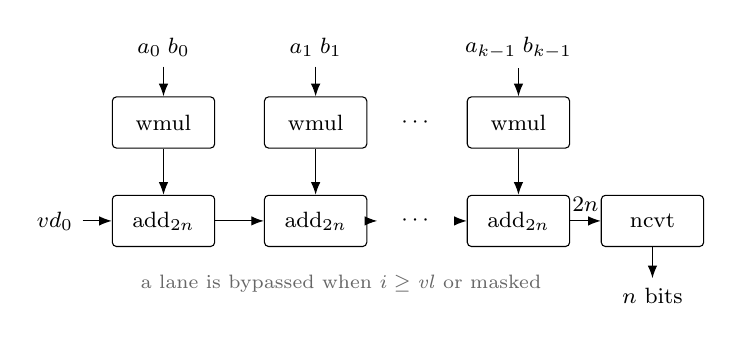
\begin{tikzpicture}[x=0.92cm, font=\footnotesize, >={Latex[length=1.6mm]},
  blk/.style={draw, rounded corners=1.5pt, minimum height=6.5mm, minimum width=13mm, align=center}]
  \foreach \i/\x in {0/0, 1/2.1, 2/4.9} {
    \node[blk] (m\i) at (\x, 0) {wmul};
    \node[blk] (a\i) at (\x,-1.25) {add$_{2n}$};
    \draw[->] (m\i) -- (a\i);
  }
  \node at (3.5, 0) {$\cdots$}; \node at (3.5,-1.25) {$\cdots$};
  \node (in0) at (0, 0.95) {$a_0\; b_0$}; \node (in1) at (2.1, 0.95) {$a_1\; b_1$};
  \node (in2) at (4.9, 0.95) {$a_{k-1}\; b_{k-1}$};
  \foreach \i in {0,1,2} \draw[->] (in\i) -- (m\i);
  \node (acc) at (-1.5,-1.25) {$vd_0$};
  \draw[->] (acc) -- (a0); \draw[->] (a0) -- (a1);
  \draw[->] (a1) -- (2.95,-1.25); \draw[->] (4.05,-1.25) -- (a2);
  \node[blk] (nc) at (6.75,-1.25) {ncvt};
  \draw[->] (a2) -- node[above] {$2n$} (nc);
  \node (y) at (6.75,-2.2) {$n$ bits};
  \draw[->] (nc) -- (y);
  \node[align=center, text=black!60] at (2.45,-2.05) {\scriptsize a lane is bypassed when $i\ge \mathit{vl}$ or masked};
\end{tikzpicture}
\caption{\code{vtdot.vv} datapath for $k$ lanes of $n$-bit elements, followed by \code{vncvt.t.t}.
Products are exact in $2n$ bits; only the additions round.}
\label{fig:dot}
\end{figure}

\subsection{Vector unit and simulator}

The vector unit \code{takum\_vec\_alu} (parameter VLEN, 64 by default) instantiates one row of ALUs per
element width and selects by SEW. Elements with $i\ge \mathit{vl}$ and masked-off elements keep the old
destination value. It is combinational; a pipelined implementation would register between the three
stages and share the multipliers of \code{vtmul.vv} and \code{vtdot.vv}.

To run whole programs we wrote an instruction-level simulator in Python. It assembles a small RV64I
subset, the RVV configuration, load/store, indexed-load and floating-point instructions needed by the
kernels, and Zvtakum; the machine fetches 32-bit words, decodes and executes them, and counts executed
instructions. IEEE~754 formats~\cite{ieee754} are modelled by a generic correctly rounded binary format (subnormals,
infinities, NaN and the five \code{fflags}); negative zero is not modelled. The takum operations call the
same oracle that verifies the RTL.

%======================================================================
\section{Results and Discussion}

\subsection{Verification}

The RTL is compared with an oracle that decodes takums with the full formula and computes in exact
rational arithmetic, sharing neither code nor method with the hardware. Table~\ref{tab:verif} summarises
the test suite; all tests pass. To check that the tests are sensitive, we injected 13 defects (for
example, dropping the sticky bit, skipping the tie-to-even rule in the narrowing, accumulating the dot
product in reverse order, ignoring the mask); every one was detected. The oracle was in turn compared with libtakum~\cite{libtakum}, the reference
implementation by the author of the format: 826\,987 vectors agree bit for bit, and 16 T32 products differ in
the last bit because libtakum multiplies in binary64, which cannot hold the 56-bit product; in all 16 the
exact result is closer to ours. The simulator is checked against
native binary16/32/64 arithmetic (160\,000 cases) and executes the 15\,000 vector-unit test vectors as
encoded instructions with identical results.

\begin{table}[t]
\caption{Verification of the RTL against the exact oracle.}
\label{tab:verif}
\centering
\begin{tabular}{@{}lr@{}}
\toprule
Test & Vectors\\
\midrule
Decoder, encoder, round trip (T8/T16 exhaustive) & 855\,408\\
ALU T8: all pairs $\times$ add, sub, mul & 196\,608\\
ALU T16, T32: edges, neighbours, random (each) & 109\,923\\
Narrowing T16$\to$T8 (all words), T32$\to$T16, T64$\to$T32 & 105\,794\\
Widening multiply T8 (all pairs), T16, T32 & 138\,818\\
Vector unit, 5 instructions, \code{vl} and mask (per SEW) & 5\,000\\
\bottomrule
\end{tabular}
\end{table}

\subsection{Hardware cost}

Table~\ref{tab:hw} gives a technology-independent synthesis (Yosys, 6-input LUT mapping). The numbers
are meant to compare blocks with each other, not as absolute area. The header decoder costs \HWHDR{} LUTs at
every width. The narrowing conversion is smaller than a decoder, which confirms that it is only a
rounding of the word. The widening multiplier is cheaper than the full ALU because it has no alignment
or normalisation shifter; at 32 bits the $28\times28$ multiplier dominates both. The combinational \code{vtdot.vv}
is the largest block, since every lane carries a double-width adder; an area-conscious design would
iterate one adder over the lanes.

\begin{table}[t]
\caption{Synthesis results in LUT6 (Yosys, generic).}
\label{tab:hw}
\centering
\begin{tabular}{lrrr}
\toprule
Block & T8 & T16 & T32\\
\midrule
Decoder & \HWDECA & \HWDECB & \HWDECC\\
Encoder & \HWENCA & \HWENCB & \HWENCC\\
ALU (add, sub, mul) & \HWALUA & \HWALUB & \HWALUC\\
Narrowing to this width (\code{vncvt.t.t}) & \HWNCA & \HWNCB & \HWNCC\\
Widening multiplier & \HWWMA & \HWWMB & \HWWMC\\
\code{vtdot.vv}, 64-bit vector (8/4/2 lanes) & \HWDOTA & \HWDOTB & \HWDOTC\\
\bottomrule
\end{tabular}
\end{table}

\subsection{Accuracy of the sparse matrix--vector product}

We compute $y=Ax$ for the nine matrices of Table~\ref{tab:mats}, stored in CSR format. Four are
generated: \emph{poisson} is the 5-point Laplacian on a $16\times16$ grid applied to a smooth mode, with
strong cancellation in every row; \emph{gauss} is random sparse with $\mathcal{N}(0,1)$ entries;
\emph{wide} has the same structure with log-uniform magnitudes; and \emph{mlp} is a pruned dense layer
(90\% zeros, weights $\mathcal{N}(0,2/\mathrm{fan\_in})$) applied to post-ReLU activations, a typical
machine-learning kernel. Four are real problems from the Harwell-Boeing collection~\cite{duff1989},
obtained from the Matrix Market~\cite{boisvert1997}: \emph{nos4} (structural analysis of a beam),
\emph{bus494} (\code{494\_bus}, admittance matrix of a 494-bus power network), \emph{west0479} (chemical
engineering, a distillation column) and \emph{bcsstk05} (structural stiffness matrix). A fifth real
matrix from the same repository, \emph{memplus} (simulation of a computer memory circuit), has 17\,758
rows, 36 times the largest of the others, and entries as small as $2^{-86}$. For the real
matrices $x$ is drawn from $\mathcal{N}(0,1)$. The data are held in binary64, rounded to each format and
multiplied by the assembly kernel in the simulator. The reference is the same product computed in
binary128 from the unrounded data, and the metric is the relative error of each row.

\begin{table}[t]
\caption{Test matrices. Top: generated; bottom: Matrix Market.}
\label{tab:mats}
\centering
\setlength{\tabcolsep}{4pt}
\begin{tabular}{@{}lcrrc@{}}
\toprule
Matrix & Size & Non-zeros & Per row & $|a_{ij}|$ range\\
\midrule
\MATTABLE
\bottomrule
\end{tabular}
\end{table}

Three kernels are compared: \emph{T}$n$ uses \code{vtdot.vv} and \code{vncvt.t.t}; \emph{FP}$n$ uses
\code{vfmul.vv} and \code{vfredosum.vs} at SEW, the usual RVV formulation; and \emph{FP}$n$\emph{w} uses
\code{vfwmul.vv}, an ordered sum at $2\,$SEW and \code{vfncvt.f.f.w}, which gives IEEE the same widened
accumulation as \code{vtdot.vv}. Table~\ref{tab:err} reports the median error and
Fig.~\ref{fig:cdf} the cumulative distributions.

\begin{table*}[t]
\caption{Median relative error of $y=Ax$ against binary128. Bold: best of each width. $\infty$: more than half
of the rows are not finite.}
\label{tab:err}
\centering
\setlength{\tabcolsep}{4.5pt}
\begin{tabular}{@{}lccccccccc@{}}
\toprule
Kernel & poisson & gauss & wide & mlp & nos4 & bus494 & west0479 & bcsstk05 & memplus\\
\midrule
\ERRTABLE
\bottomrule
\end{tabular}
\end{table*}

\begin{figure*}[t]
\centering
\begin{tikzpicture}
\begin{groupplot}[
  group style={group size=5 by 2, horizontal sep=4mm, vertical sep=11mm, ylabels at=edge left,
               yticklabels at=edge left, xlabels at=edge bottom},
  width=0.232\textwidth, height=36mm,
  xmode=log, xmin=1e-10, xmax=1e2, ymin=0, ymax=1,
  xtick={1e-10,1e-8,1e-6,1e-4,1e-2,1e0,1e2},
  xticklabels={,$10^{-8}$,,$10^{-4}$,,$10^{0}$,},
  xlabel={relative error}, ylabel={fraction of rows},
  grid=major, grid style={black!12},
  tick label style={font=\scriptsize}, label style={font=\footnotesize}, title style={font=\footnotesize, yshift=-1.5mm},
  cycle list={}, every axis plot/.append style={line width=0.8pt},
  legend style={font=\scriptsize, legend columns=6, /tikz/every even column/.append style={column sep=3mm}}]
\matplot{poisson}
\matplot{gauss}
\matplot{wide}
\matplot{mlp}
\matplot{nos4}
\matplot{bus494}
\matplot{west0479}
\matplot{bcsstk05}
\matplot[legend to name=cdfleg]{memplus}
\legend{T8, FP8w, T16, FP16w, T32, FP32w}
\end{groupplot}
\end{tikzpicture}\\[1.5mm]
\pgfplotslegendfromname{cdfleg}
\caption{Cumulative distribution of the relative error of $y=Ax$ over the rows of each matrix, against
binary128. Solid: takum with \code{vtdot.vv}; dashed: IEEE with widened accumulation. Curves to the left
are better. A curve that does not reach 1 has non-finite results.}
\label{fig:cdf}
\end{figure*}

\emph{32 bits.} T32 has the lowest median error on all nine matrices, by a factor of \RATA{} to
\RATB{} with respect to FP32w. Most operands have $r\le3$, so T32 carries 24 to 27 fraction bits against
the 23 of binary32; the smallest gain is on \emph{bcsstk05}, whose entries reach $2^{22}$ ($r=4$, 23
bits).

\emph{16 bits.} T16 is better than FP16w on \emph{poisson}, \emph{gauss}, \emph{mlp}, \emph{nos4} and
\emph{west0479}, where most data are within a few binades of 1 and T16 has 10 or 11 fraction bits. It is
worse on \emph{wide} (\WIDET{} against \WIDEF{}), \emph{bus494} (\BUST{} against \BUSF{}) and
\emph{memplus} (\MEMTS{} against \MEMFS{}): magnitudes around $2^{\pm10}$ need $r=3$, leaving 8
fraction bits against the 10 of binary16. This is the
cost of tapering, and it shows only while binary16 still has range. Beyond it the comparison inverts:
binary16 returns infinities or NaN in \NFWESTH{} of the 479 rows of \emph{west0479} and in \NFBCSH{} of
the 153 rows of \emph{bcsstk05}, where T16 is finite everywhere with a median error of \BCSTSIXTEEN.

\emph{8 bits.} Where the 8-bit float stays in range it is the more precise format, by a factor of 1.5 to
3 in the median: T8 has three fraction bits only in $[0.5,2)$, two in the neighbouring binades and fewer
beyond. Both are too coarse for \emph{poisson}, where the cancellation amplifies the input rounding to
errors above 100\% in most rows. The advantage of T8 is range. FP8w returns infinities or NaN in
\FPEIGHTBAD{} of 256 rows of \emph{wide}, \NFBUS{} of 494 of \emph{bus494}, \NFWEST{} of 479 of
\emph{west0479} and all \NFBCS{} of \emph{bcsstk05}, and no kernel can avoid it because the data
themselves are out of range. On \emph{memplus} the limit is at the other end: entries down to $2^{-86}$
underflow the 8-bit float, whose result is off by 100\% or more in \MEMFEBAD{} of the \MEMROWS{} rows,
against \MEMTEBAD{} for T8, although the median error of the float is lower. T8 returns a finite result for every row of
every matrix.

\emph{Effect of the widened accumulation.} Repeating the takum product with \code{vtmul.vv} and
\code{vtadd.vv} at SEW, the median error grows by a factor of 1.2 to 2.3. The final narrowing of
\code{vtdot.vv} is a single rounding, so the remaining error is dominated by the rounding of the inputs:
on the eight matrices without systematic cancellation, the best possible result (the correctly rounded
reference) is less than 3 times more accurate.

\subsection{Instruction count}

\begin{figure}[t]
\footnotesize
\begin{verbatim}
inner:
  vsetvli    t3, t2, e16, m1, ta, ma
  vle32.v    v8, (a2)        # column offsets
  vle16.v    v1, (a3)        # values of the row
  vluxei32.v v2, (a4), v8    # gather x[col]
  vtdot.vv   v4, v1, v2      # T32 acc += v1 . v2
  ...                        # 6 pointer/loop instr.
done:
  vsetvli    zero, s1, e16, m1, ta, ma  # vl=1
  vncvt.t.t  v5, v4          # T32 -> T16
  vse16.v    v5, (a5)

# IEEE with the same widened accumulation,
# in place of vtdot.vv:
  vfwmul.vv    v6, v1, v2    # binary32 products
  vsetvli      zero, t3, e32, m2, ta, ma
  vfredosum.vs v4, v6, v4
\end{verbatim}
\caption{Inner loop and row epilogue of the CSR kernel for 16-bit elements.}
\label{fig:asm}
\end{figure}

Fig.~\ref{fig:asm} shows the kernel and Table~\ref{tab:instr} counts the executed instructions. The inner
loop has 11 instructions per strip with \code{vtdot.vv}, 12 with \code{vfmul}/\code{vfredosum}, and 13
with widening, which needs a second \code{vsetvli} per strip because the products and the reduction use
different element widths. \code{vtdot.vv} produces the widened sum without changing \code{vtype}. Over
all matrices and element widths, the saving against the IEEE kernel of the same accuracy class (FPw) is
\SAVEWLO{} to \SAVEWHI\% at VLEN${}=128$; against the plain kernel it is 0 to \SAVEPHI\%. The saving
grows with the number of non-zeros per row. When a row fits in a single strip the per-row overhead (12 or
13 instructions) dominates and the takum kernel executes as many instructions as the plain IEEE kernel,
the fused instruction paying for the final conversion; the real matrices other than \emph{bcsstk05},
with 3 to 7 non-zeros per row, are at or near this case.

\begin{table}[t]
\caption{Executed instructions for $y=Ax$, SEW${}=16$, VLEN${}=128$. \emph{wide} has the structure of
\emph{gauss}.}
\label{tab:instr}
\centering
\setlength{\tabcolsep}{3.2pt}
\begin{tabular}{@{}lrrrrrr@{}}
\toprule
 & nnz/ & & & & \multicolumn{2}{c}{Saving vs.}\\
Matrix & row & Zvtakum & FP & FPw & FP & FPw\\
\midrule
\INSTRTABLE
\bottomrule
\end{tabular}
\end{table}

\subsection{Instruction-set and CSR complexity}

Beyond instruction counts, the takum unit removes control state and whole instruction classes.

\emph{Control and status.} RVV floating-point instructions read the rounding mode \code{frm} (3 bits,
five modes) and accumulate into \code{fflags} (5 bits), both in \code{fcsr}, which must be saved,
restored and renamed by an out-of-order core. Takum arithmetic defines one rounding mode and signals
exceptional results in-band with NaR, so Zvtakum reads and writes no CSR other than \code{vl} and
\code{vtype}. In our runs the IEEE kernels raised flags in up to \FLAGPCT\% of the element operations
(\FLAGWHERE) and FP8 on \emph{wide} ended with inexact, underflow, overflow and invalid set; the
takum kernels have no such side channel to maintain.

\emph{Instructions that become integer operations.} Since takum words order like two's complement
integers and negation is the integer negation, the six vector floating-point compares
(\code{vmfeq}, \code{vmfne}, \code{vmflt}, \code{vmfle}, \code{vmfgt}, \code{vmfge}), minimum and
maximum (\code{vfmin}, \code{vfmax}), the three sign-injection instructions (\code{vfsgnj},
\code{vfsgnjn}, \code{vfsgnjx}) and \code{vfclass} need no takum counterpart: the existing integer
compares, \code{vmin}/\code{vmax} and \code{vneg} already give the right answer, with the NaR pattern
ordered below every number. IEEE needs dedicated instructions because of signed zeros, unordered NaNs
and sign-magnitude encoding.

\emph{Conversions.} Narrowing is a rounding of the word (Table~\ref{tab:hw}) and widening is appending
zero bits, which is exact. The three takum widths therefore form one
format family, whereas E4M3, E5M2, binary16, bfloat16 and binary32 each need their own conversion
logic to every other.

\subsection{Limitations}

The datapath is combinational and was not placed and routed; we do not report timing or a comparison
with an IEEE ALU of the same width. T16 and T32 are verified by directed and random sampling rather
than exhaustively. All matrices but \emph{memplus} are small (at most 494 rows) and, for the real ones, $x$ is random; the simulator counts
instructions, not cycles.
The 8-bit float is an E4M3 layout under IEEE~754 rules, with infinities. We chose it because the comparison
is against the IEEE~754 standard, which defines no 8-bit format, and this keeps FP8, FP16 and FP32 one
arithmetic at three widths; it differs from OFP8, whose E4M3 has no infinities, so part of the non-finite
results reported for FP8 would be saturated values there.

%======================================================================
\section{Conclusion}

We implemented and verified a takum vector datapath for RISC-V and evaluated it at the instruction
level. Three properties of the format translate directly into hardware and ISA simplifications: the
fixed 12-bit header gives one decoder for all widths; monotonic bit patterns turn rounding, narrowing,
comparison and negation into integer operations; and the absence of flags and rounding modes removes
the floating-point CSR. Numerically, takums are the better choice at 32 bits and, for data near unit
scale, at 16 bits; at 8 bits their value is range rather than precision. A fused dot product with a
double-width accumulator fits the format well, because products are exact at double width, and shortens
the sparse matrix--vector kernel. Future work includes a pipelined implementation with timing results,
a like-for-like area comparison with IEEE units, and a wider set of large matrices.

%======================================================================
\begin{thebibliography}{00}
\bibitem{hunhold2025avx} L.~Hunhold, ``Streamlining SIMD ISA extensions with takum arithmetic: A case
study on Intel AVX10.2,'' in \emph{Proc.\ 14th Int.\ Conf.\ Modern Circuits and Systems Technologies
(MOCAST)}, 2025, pp.~1--6.
\bibitem{hunhold2024takum} L.~Hunhold, ``Beating posits at their own game: Takum arithmetic,'' in
\emph{Next Generation Arithmetic (CoNGA 2024)}, LNCS 14666. Springer, 2024, pp.~1--51.
\bibitem{ofp8} P.~Micikevicius \emph{et al.}, ``OCP 8-bit floating point specification (OFP8),'' Open
Compute Project, 2023.
\bibitem{gustafson2017} J.~L. Gustafson and I.~Yonemoto, ``Beating floating point at its own game:
Posit arithmetic,'' \emph{Supercomputing Frontiers and Innovations}, vol.~4, no.~2, pp.~71--86, 2017.
\bibitem{positstd} Posit Working Group, ``Standard for posit arithmetic (2022),'' 2022.
\bibitem{hunhold2024codec} L.~Hunhold, ``Design and implementation of a takum arithmetic hardware codec
in VHDL,'' arXiv:2408.10594, 2024.
\bibitem{rvv} RISC-V International, ``RISC-V `V' vector extension,'' version 1.0, 2021.
\bibitem{hunhold2025solvers} L.~Hunhold and J.~Quinlan, ``Evaluation of bfloat16, posit, and takum
arithmetics in sparse linear solvers,'' in \emph{Proc.\ IEEE Symp.\ Computer Arithmetic (ARITH)}, 2025,
arXiv:2412.20268.
\bibitem{ieee754} \emph{IEEE Standard for Floating-Point Arithmetic}, IEEE Std 754-2019, 2019.
\bibitem{libtakum} L.~Hunhold, ``libtakum,'' version 2.0.0, 2025. [Online]. Available:
\url{https://github.com/takum-arithmetic/libtakum}
\bibitem{duff1989} I.~S. Duff, R.~G. Grimes, and J.~G. Lewis, ``Sparse matrix test problems,''
\emph{ACM Trans.\ Math.\ Softw.}, vol.~15, no.~1, pp.~1--14, 1989.
\bibitem{boisvert1997} R.~F. Boisvert, R.~Pozo, K.~Remington, R.~F. Barrett, and J.~J. Dongarra, ``Matrix
Market: A web resource for test matrix collections,'' in \emph{Quality of Numerical Software}.
Chapman \& Hall, 1997, pp.~125--137.
\end{thebibliography}

\end{document}
